\documentclass[12pt]{article}
\usepackage{graphicx}
\usepackage{float}
\usepackage{CJK}


\title{\bf{Paper Reading for\\ The Weighted Center of A Tree}}
\date{}

\begin{document}
\begin{CJK}{UTF8}{bkai}

\maketitle

\section{問題定義}
~~~~給予一個 {\it tree} $T=(V,E)$。 $T$ 上的每一個 {\it node} 都有一個非負的 {\it weight}
且每一個 {\it edge} 都有一個非負的 {\it length}。假設 $x$ 為 $T$ 上面的一 node , $x$
 可能屬於 $V$ , 也可能存在在某個 edge 上。$d(i,j)$ 表示 node $i$ 和 node $j$ 之間的最
短距離, $w_i$ 為 node $i$ 上的 weight 。$r(x)$的正式定義如下:

\begin{equation}
r(x)=max\{w_id(x,i)|i\in V\}
\end{equation}

本問題想要求出一個 node $x$ ,使得 $r(x)$ 為最小值。

\section{定義}

\begin{enumerate}
\item {\it centroid} :存在一個 node $c$ 使得 $r(c)$ 為最小值。
\item $V_j(x)$ :收集 node $i$ 且 node $i$ 與 node $x$ 之間的 {\it simple path} 存在
 node $j$ 。
\item $T_j(x)$ : $T$ 上面的一個 {\it subtree} 且點集合為 $V_j(x) \cup \{x\}$ 。
\item $r_j(x)$ : max$\{w_id(x,i)|i \in V_j(x)\}$
\end{enumerate}

\section{方法說明}

\begin{enumerate}

\item 找出一個 node $c$ 且與 $c$ 鄰近的 nodes 為 $j_1$ 、 $j_2$ 、...、 $j_m$ 。 $T$ 可分成
 $m$ 個 subtree $T_{j_1}(c)$ 、...、 $T_{j_m}(c)$ ,每個 subtree 的 node 個數 $|V_{j_i}(c)|$ 小
於等於 $|V|/2$ , $i \in \{1,2,...,m\}$ 。

\item 計算 $r_{j_1}(c)$ 、 $r_{j_2}(c)$ 、...、 $r_{j_m}(c)$ ,這 $m$ 個值取最大當 $r(c)$ 。

\item 當存在兩個 nodes $j_k \neq  j_l$ 使得 $r_{j_k}(c)=r_{j_l}(c)=r(c)$ ,則 $c$ 為 $T$ 的
 centroid 。

\item 假設只有一 node $j$ 使得 $r_{j}(c)=r(c)$ ,所以我們知道 centroid 存在在 $T_j(c)$ 。

\item 在 $T_j(c)$ 之外的點,兩兩湊成一對 $(u_1,v_1)$ 、 $(u_2,v_2)$ 、...、 $(u_s,v_s)$ 。

\item 不失一般性,假設每一對 $(u,v)$ 滿足此不等式 $w_ud(u,c) \geq w_vd(v,c)$ 。若 $w_u \geq w_v$
, node $v$ 就刪除;若不是,則 $t_{uv}=\frac{w_ud(u,c)-w_vd(v,c)}{w_v-w_u}$ 。

\item 所有配對 $(u_1,v_1)$ 、...、 $(u_s,v_s)$ 分別的 $t_{u_1v_1}$ 、...、 $t_{u_sv_s}$都求出後,
從中找出中位數 $t_m$ 。

\item 在 $T_j(c)$ 裡面找出所有 nodes $y$ 使得 $d(c,y)=t_m$ 。假設找到 $y_1$ 、...、 $y_n$ ,這
$n$ 個 nodes 有可能在邊上 。

\item 收集所有的 nodes $z$ 且 $d(c,z)\geq t_m$ ,則這些點集就是 $p$ 個 subtree $T_1$ 、...、 $T_p$
 的聯集,如 Figure 1 。

%Fig 1
\begin{figure}[H]
\centering
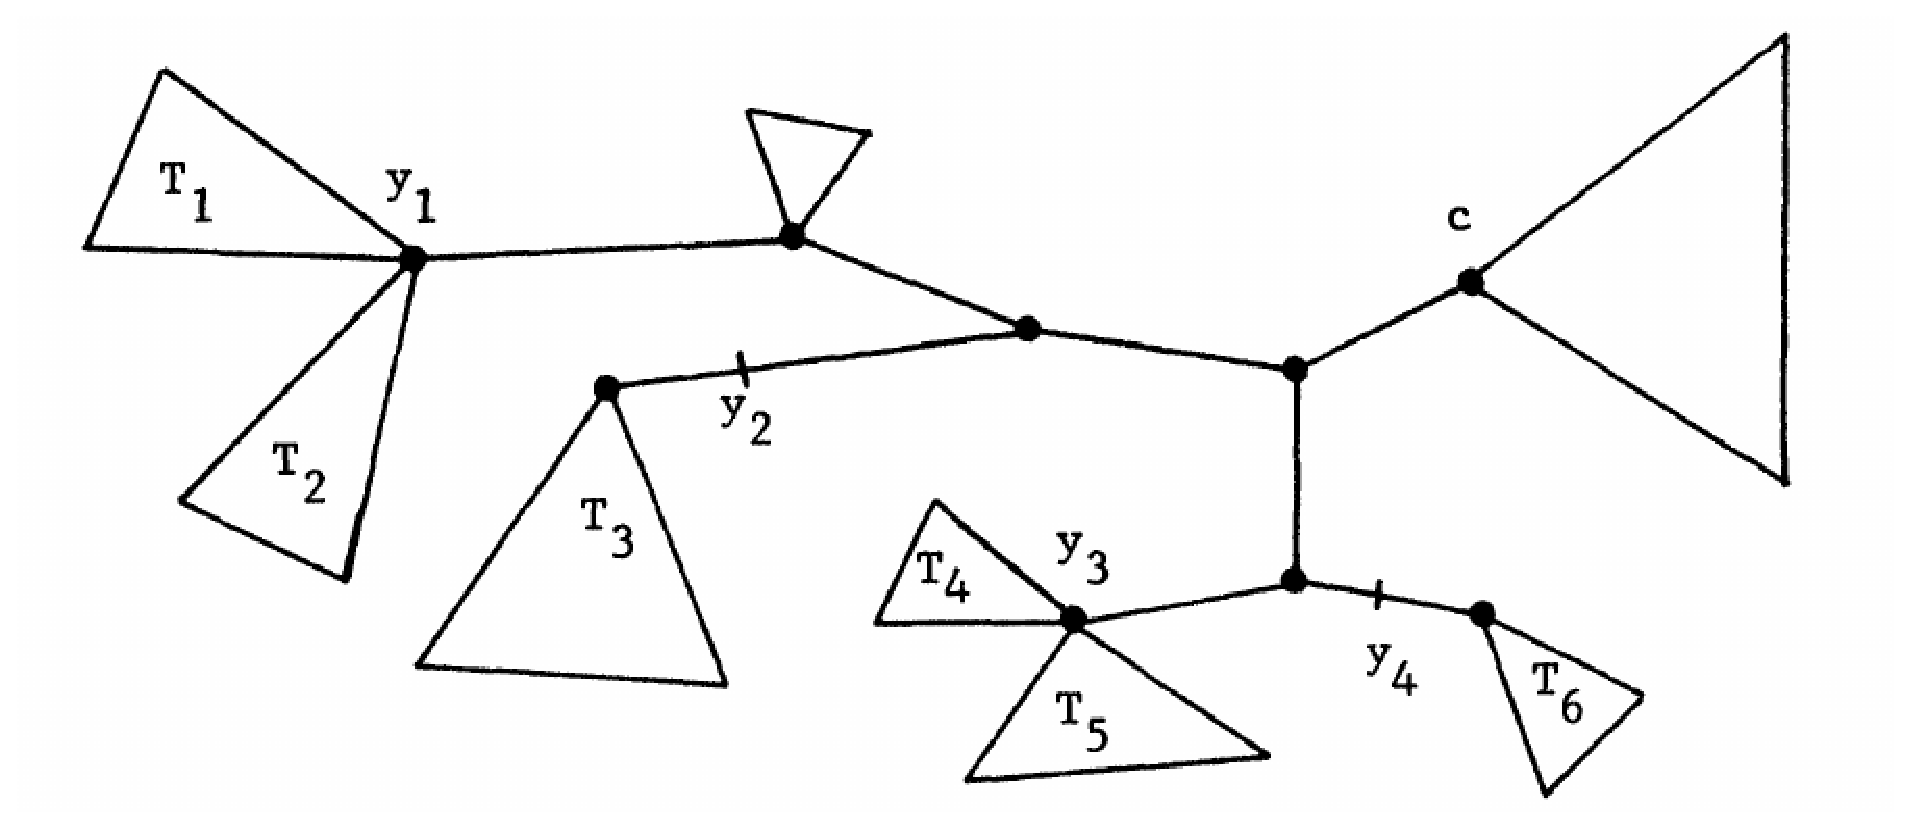
\includegraphics[scale=0.3]{fig1.eps}
\caption{}
\end{figure}

\item 求出各 subtree $T_i$ 的 $R(i)=max\{w_jd(i,j)|j \in V(T_i)\}$ 且 $i \in {1,...,p}$ ,其中最大值
為 $R$ 。

\item 若存在兩個 subtree $T_i$ 和 $T_j$ 使得 $R(i)=R(j)=R$ ,則 $\{z|d(c,z)\geq t_m\}$ 不存在 centroid
;若只有一個 subtree $T_i$ 使得 $R(i)=R$,則 centroid 存在在 $T_i$ 之中。

\item 假設已知 centroid 落在 $\{z|d(c,z)<t_m\}$ 之中,則當 $t_{uv}\geq t_m$ 時,可以把 node $v$ 刪掉;
若 centroid 落在 $\{z|d(c,z)\geq t_m\}$ 之中,則當 $t_{uv} < t_m$ 時, 可以把 node $u$ 刪掉。 

\item 重複上述步驟 $1\sim12$ 直到 node 數夠少,就直接暴力解。

\end{enumerate}

\section{例子}

~~~~以 Figure 2 為例子,黑色數字代表 node 上面的 weight ,紅色數字代表 edge 上面的 weight 。這邊的 nodes
的 weight 有 2 、5 、 6 、 7 、 9 、 10 和 18 ,令這些 nodes 分別為 $v_1$ 、$v_2$ 、$v_3$ 、$v_4$ 、$v_5$
、 $v_6$  和 $v_7$。

%Fig 2
\begin{figure}[H]
\centering
\includegraphics[scale=0.3]{fig2.eps}
\caption{}
\end{figure}

我們選擇 $v_2$ 作為暫時的 centroid,與此 centroid 相鄰的為 $v_3$ 、 $v_4$ 和 $v_6$ 的 nodes ,則
$r_{v_3}(v_2)=18$ 、 $r_{v_4}(v_2)=198$、 $r_{v_6}(v_2)=50$ ,如 Figure 3 所示。

%Fig 3
\begin{figure}[H]
\centering
\includegraphics[scale=0.3]{fig3.eps}
\caption{}
\end{figure}

因此,我們可以知道真正的 centroid 在 $T_{v_4}(v_2)$ ,所以我們這次取 $v_3$ 和 $v_6$ 的 nodes 做為一對,如
Figure 4 所示 。

%Fig 4
\begin{figure}[H]
\centering
\includegraphics[scale=0.3]{fig4.eps}
\caption{}
\end{figure}

比較一下就發現 $10 \times 5 > 6 \times 3$ 且 $10 > 6$ ,所以我們要把 $v_3$ 刪除,其結果如 Figure 5 。

%Fig 5
\begin{figure}[H]
\centering
\includegraphics[scale=0.3]{fig5.eps}
\caption{}
\end{figure}

這次一樣取 $v_2$ 的 node 做暫時的 centroid ,與 $v_2$ 相鄰的 nodes 為 $v_4$ 和 $v_6$ ,所以 $r_{v_4}(v_2)=198$
且 $r_{v_6}(v_2)=50$ ,如 Figure 6 所示。

%Fig 6
\begin{figure}[H]
\centering
\includegraphics[scale=0.3]{fig6.eps}
\caption{}
\end{figure}

因此,我們可以知道真正的 centroid 在 $T_{v_4}(v_2)$ ,所以我們這次取 $v_1$ 和 $v_6$ 做為一對,如 Figure 7 所示 。

%Fig 7
\begin{figure}[H]
\centering
\includegraphics[scale=0.3]{fig7.eps}
\caption{}
\end{figure}

比較一下就發現 $10 \times 5 > 2 \times 7$ 且 $10 > 2$ ,所以我們要把 $v_1$ 刪除,其結果如 Figure 8 。

%Fig 8
\begin{figure}[H]
\centering
\includegraphics[scale=0.3]{fig8.eps}
\caption{}
\end{figure}

這次取 $v_4$ 做暫時的 centroid ,與 $v_4$ 相鄰的 $v_2$ 、 $v_5$ 和 $v_7$ ,所以 $r_{v_2}(v_4)=70$ 、 $r_{v_5}(v_4)=90$ 且
$r_{v_7}(v_4)=162$ ,如 Figure 9 所示。

%Fig 9
\begin{figure}[H]
\centering
\includegraphics[scale=0.3]{fig9.eps}
\caption{}
\end{figure}

因此,我們可以知道真正的 centroid 在 $T_{v_7}(v_4)$ ,所以我們取 $v_2$ 和 $v_6$ 做為一對,如 Figure 10 所示 。

%Fig 10
\begin{figure}[H]
\centering
\includegraphics[scale=0.3]{fig10.eps}
\caption{}
\end{figure}

比較一下就發現 $10 \times 7 > 5 \times 2$ 且 $10 > 5$ ,所以我們要把 $v_2$ 刪除,其結果如 Figure 11 。

%Fig 11
\begin{figure}[H]
\centering
\includegraphics[scale=0.3]{fig11.eps}
\caption{}
\end{figure}

取 $v_4$ 做暫時的 centroid ,與 $v_4$ 相鄰的 nodes 為 $v_5$ 、 $v_6$ 和 $v_7$ ,所以 $r_{v_5}(v_4)=90$ 、 $r_{v_6}(v_4)=70$
且 $r_{v_7}(v_4)=162$ ,如 Figure 12 所示。

%Fig 12
\begin{figure}[H]
\centering
\includegraphics[scale=0.3]{fig12.eps}
\caption{}
\end{figure}

因此,我們可以知道真正的 centroid 在 $T_{v_7}(v_4)$ ,所以我們取 $v_5$ 和 $v_6$ 做為一對,如 Figure 13 所示 。

%Fig 13
\begin{figure}[H]
\centering
\includegraphics[scale=0.3]{fig13.eps}
\caption{}
\end{figure}

比較一下就發現 $9 \times 10 > 10 \times 7$ 且 $10 > 9$ ,所以 $t_{v_5v_6}=\frac{90-70}{10-9}=20$ 。不過,由 Figure 13
可以知道真正的 centroid 一定與 $v_4$ 的最短距離小於 20 ,所以把 $v_6$ 刪掉, 其結果如 Figure 14 。

%Fig 14
\begin{figure}[H]
\centering
\includegraphics[scale=0.3]{fig14.eps}
\caption{}
\end{figure}

從 Figure 14 可知 ,點數已經夠少了,可以直接暴力解。取 $v_4$ 為暫時的 centroid ,解開以下等式:

\begin{equation}
w_{v_5}d(v_4,v_5)+t \times w_{v_5}=w_{v_7}d(v_4,v_7)-t \times w_{v_7}
\end{equation}

最後 $t=\frac{8}{3}\approx 2.67$ ,所以真正的 centroid $c^*$ 位置如 Figure 15 所示。

%Fig 15
\begin{figure}[H]
\centering
\includegraphics[scale=0.3]{fig15.eps}
\caption{}
\end{figure}

\section{時間複雜度分析}

~~~~由上面方法說明可以知道,執行步驟 $1\sim12$ 一次的時間只要 $O(|V|)$ ,而且每執行一次至少會刪掉 $|V|/8$
個 nodes。因此,整體的時間複雜度 $T(n)\leq T(n/8)+O(n)=O(n)$ (假設 $|V|=n$)。


\end{CJK}

\end{document}
